\providecommand{\main}{..}		% Override relative path to the main file (already set in main file)
\documentclass[../InterneDSLs.tex]{subfiles}
\begin{document}

\section{Hauptteil}
Für die Verarbeitung der \ac{EBNF}-Grammatiken wird ANTLR4 verwendet, der Parser und Lexer für Java generieren kann.

\subsection{Parser}
Als Parser-Generator wurde ANTLR4 verwendet, der Parser zu einer EBNF-Grammatik in Java generieren kann. Dafür verwendet ANTLR aber eine unübliche Syntax, die sich an einer alten EBNF-Variante orientiert.

Der von ANTLR generierte Parser wird von einem Listener erweitert, der aus den EBNF-Konstrukten (die praktisch Strings entprechen) einen Baum aus eigenen Klassen generiert. Dadurch wird eine Typ-Sicherheit hergestellt, die durch die EBNF selbst nicht gegeben ist.

\subsubsection{Erzeugung von Typen aus der Grammatik}


\subsection{Abbildung von EBNF auf Interfaces}
Zuerst wird die in EBNF geschriebene Grammatik in einen Baum aus Java-Objekten transformiert. Dadurch wird eine Typ-Sicherheit hergestellt und Methoden implementiert werden, die das Traversieren des Baumes vereinfachen. Abbildung~\ref{FIG:TypesBNF} zeigt die Typen und ihre Beziehungen untereinander.

\begin{figure}[ht]
\centering
\includegraphics[width=\linewidth]{\main/10_Pictures/BNF-Types}
\caption{Typen des BNF-Baumes}
\label{FIG:TypesBNF}
\end{figure}

\subsubsection{Parse-Tree}


\subsubsection{Abbildung von Kanten auf Interfaces}
Um die Interfaces generieren zu können, müssen die Kanten der Graphen zwischen den Scopes, auf Interfaces abgebildet werden.

\paragraph{Kante mit einem Knoten}
Im einfachsten Fall von einer Kante, die nur einen Sequenz-Knoten beinhaltet, kann man den ein Interface mit dem Namen des Knotens und dem nächsten Scope als Rückgabewert erstellen. Grafik~\ref{FIG:OneElementNode} zeigt, wie eine Abbildung aussehen kann.
\begin{figure}[ht]
\centering
  \begin{subfigure}[c]{0.49\textwidth}
    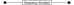
\includegraphics[width=.95\linewidth]{\main/10_Pictures/Nodes_one-element}
    \caption{Diagramm eines Sequenz-Knotens}
    \label{FIG:DiagramOneElementNode}
  \end{subfigure}
  \begin{subfigure}[c]{0.49\textwidth}
    \lstinputlisting[language=Java]{Scope_one-element.java}
    \caption{Java-Interface aus einem Sequenz-Knoten}
    \label{FIG:JInterfaceOneElementNode}
  \end{subfigure}
  \caption{Diagramm und Interface eines Sequenz-Knotens}
  \label{FIG:OneElementNode}
\end{figure}

\paragraph{Optionale Kante mit einem Knoten}
Falls man einen Knoten überspringen kann (bzw. optional ist), muss man vom folgenden Scope (Listing~\ref{FIG:JInterfaceOptionalNode}) erben, um dessen Methoden aufrufen zu können und damit die eigene(n) auslassen zu können.
\begin{figure}[ht]
\centering
  \begin{subfigure}[c]{0.49\textwidth}
    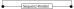
\includegraphics[width=.95\linewidth]{\main/10_Pictures/Nodes_optional}
    \caption{Diagramm eines optionalen Sequenz-Knotens}
    \label{FIG:DiagramOptionalNode}
  \end{subfigure}
  \begin{subfigure}[c]{0.49\textwidth}
    \lstinputlisting[language=Java]{Scope_optional.java}
    \caption{Java-Interface aus einem optionalen Sequenz-Knoten}
    \label{FIG:JInterfaceOptionalNode}
  \end{subfigure}
  \caption{Diagramm und Interface eines optionalen Sequenz-Knotens}
  \label{FIG:OptionalNode}
\end{figure}

\paragraph{Kante mit Alternativen}
Falls eine Kante mehrere Alternativen enthält, können die alternativen je als eine Methode in einem Interface implementiert werden, die jeweils den folgenden Scope zurück geben (siehe Abbildung~\ref{FIG:AlternativeNode}).
\begin{figure}[ht]
\centering
  \begin{subfigure}[c]{0.49\textwidth}
    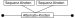
\includegraphics[width=.95\linewidth]{\main/10_Pictures/Nodes_alternative}
    \caption{Diagramm alternativer Knoten}
    \label{FIG:DiagramAlternativeNode}
  \end{subfigure}
  \begin{subfigure}[c]{0.49\textwidth}
    \lstinputlisting[language=Java]{Scope_alternative.java}
    \caption{Java-Interface aus alternativen Knoten}
    \label{FIG:JInterfaceAlternativeNode}
  \end{subfigure}
  \caption{Diagramm und Interface alternativer Knotens}
  \label{FIG:AlternativeNode}
\end{figure}

\paragraph{Kante mit Schleife}
Eine Wiederholung wird mit einem Schleifen-Knoten modelliert, der einen Sequenz-Knoten beinhaltet. Für eine Wiederholung, die kein Vorkommen erlaubt, reicht ein Scope, der vom Folge-Scope erbt; damit kann der Methodenaufruf vom Schleifen-Scope übersprungen werden.

Falls die Wiederholung mindestens ein Vorkommen voraussetzt muss ein zusätzlichen Interface eingeführt werden, das dieselbe Methode deklariert und nicht vom Folge-Interface erbt, um einen Methodenaufruf zu erzwingen (Listing~\ref{FIG:JInterfaceLoopNode}).
\begin{figure}[ht]
\centering
  \begin{subfigure}[c]{0.49\textwidth}
    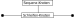
\includegraphics[width=.95\linewidth]{\main/10_Pictures/Nodes_loop}
    \caption{Diagramm eines Schleifen-Knotens}
    \label{FIG:DiagramLoopNode}
  \end{subfigure}
  \begin{subfigure}[c]{0.49\textwidth}
    \lstinputlisting[language=Java]{Scope_loop.java}
    \caption{Java-Interface aus einem Schleifen-Knoten}
    \label{FIG:JInterfaceLoopNode}
  \end{subfigure}
  \caption{Diagramm und Interface eines Schleifen-Knotens}
  \label{FIG:LoopNode}
\end{figure}

\paragraph{Sequenz von Knoten}
Tritt eine Sequenz von Knoten auf, muss für jeden Knoten ein Interface mit einer Methode generiert werden, um die Aufruf-Reihenfolge zu gewährleisten. Abbildung~\ref{FIG:SequenceNode} zeigt ein Beispiel mit zwei Knoten in einer Sequenz.
\begin{figure}[ht]
\centering
  \begin{subfigure}[c]{0.49\textwidth}
    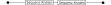
\includegraphics[width=.95\linewidth]{\main/10_Pictures/Nodes_sequence}
    \caption{Diagramm einer Sequenz von Knoten}
    \label{FIG:DiagramSequenceNode}
  \end{subfigure}
  \begin{subfigure}[c]{0.49\textwidth}
    \lstinputlisting[language=Java]{Scope_sequence.java}
    \caption{Java-Interfaces aus einer Sequenz von Knoten}
    \label{FIG:JInterfaceSequenceNode}
  \end{subfigure}
  \caption{Diagramm und Interface einer Sequenz von Knotens}
  \label{FIG:SequenceNode}
\end{figure}

\paragraph{Probleme}
\begin{itemize}
	\item Benamung der Scopes und Knoten
	\item Bestimmung des Start-Scopes
	\item Abbildung von Lexer-Regeln auf Typen der Wirtssprache
\end{itemize}


\subsection{Sprachdesign}


\subsubsection{Einschränkungen}


\end{document}
